\documentclass[12pt, xcolor={dvipsnames}, aspectratio = 169, sans, mathserif]{beamer}

\usepackage{fontspec}
\usepackage{fontawesome5}
\usepackage{mathrsfs}
\usepackage{amsmath, amssymb}
\usepackage{braket}
\usepackage{graphicx}
\usepackage{hyperref}
\usepackage[absolute,overlay]{textpos}
\usepackage[font=tiny, skip=0.5pt]{caption}

\captionsetup[figure]{labelformat=empty}

% Define the custom theme
\mode<presentation>

% \usefonttheme{serif}
% \setmainfont{Roboto}

\setbeamertemplate{footline}[frame number]
\setbeamertemplate{caption}[default]
\setbeamertemplate{navigation symbols}{}

\setbeamerfont{footnote}{size=\tiny}


% Some custom commands
\newenvironment{List}[2]
{\begin{textblock}{#1}#2
\begin{itemize}}
{\end{itemize}
\end{textblock}}

\newenvironment{Pic}[2]
{\begin{textblock}{#1}#2
\begin{figure}}
{\end{figure}
\end{textblock}}

%\newcommand{\BeamerCite}[1]{{\tiny \footfullcite{#1}}}

\newcommand{\NewCaption}[3]{\caption{{#1}, \textcolor{blue}{\href{#2}{#3}}}}

% Title of the slides
\title{Utilizing Deep Neural Networks for the Extraction of Drell-Yan Angular Coefficients in $pp$ Collisions with a 120 GeV Beam Energy}
% \subtitle{Subtitle}
\author{Dinupa Nawarathne}
\institute{New Mexico State University \\
  Representing the FermiLab SeaQuest/E906 Collaboration
}

\date{APS-DNP-2023, November 29, 2023}

\titlegraphic{

\includegraphics[height=0.8cm]{imgs/Fermilab_logo.svg.png}

\includegraphics[height=0.8cm]{imgs/NMSU_logo.jpg}

\includegraphics[height=0.8cm]{imgs/SeaQuest.jpg}

\includegraphics[height=0.8cm]{imgs/DOE.png}
}


\begin{document}

\begin{frame}
  \maketitle
\end{frame}

\begin{frame}
    \frametitle{Table of Contents}
    \tableofcontents
\end{frame}

\section{Physics Motivation}
\subsection{Internal Structure of the Proton \& Transverse Momentum Distributions}

\begin{frame}
\frametitle{Internal Structure of the Proton \& Transverse Momentum Distributions}

\begin{Pic}{6.}{(0.1, 2.0)}
  \NewCaption{J. Ashman et al. }{https://www.sciencedirect.com/science/article/pii/0370269388915237}{DOI:10.1016/0370-2693(88)91523-7}
  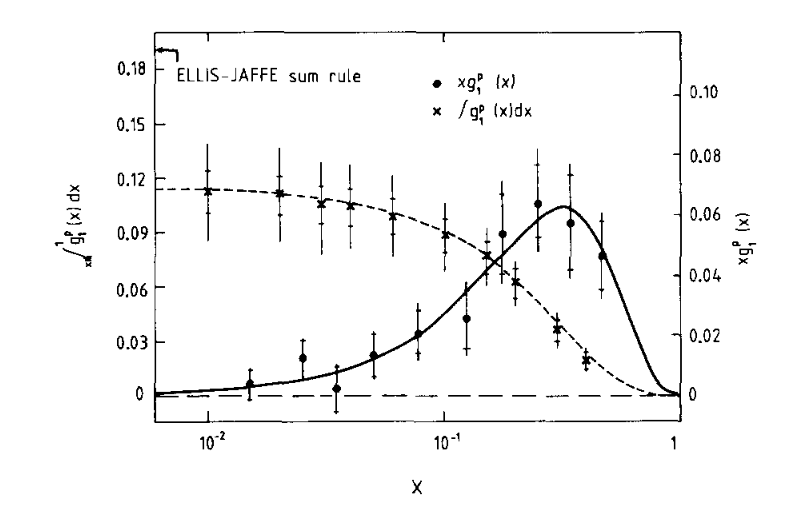
\includegraphics[width=6.cm]{imgs/EMC.png}
\end{Pic}

\begin{Pic}{4.5}{(6., 1.)}
  \NewCaption{K. F. Liu}{https://arxiv.org/abs/2112.08416}{arXiv:2112.08416}
  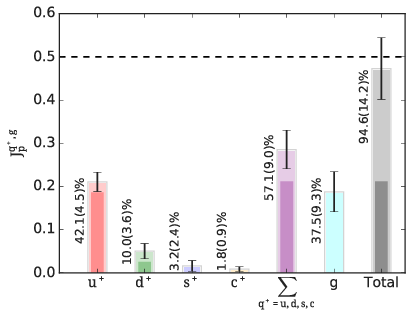
\includegraphics[width=4.5cm]{imgs/J_vbar_211.png}
\end{Pic}

\begin{List}{5.}{(10.6, 2.)}

  \item Proton is a spin $\frac{1}{2}$ fermion.

  \item Total spin of the proton $\rightarrow$ internal structure of proton.

\end{List}

\begin{Pic}{6.}{(9.5, 7.2)}
  \NewCaption{A. Accardi et al}{https://arxiv.org/abs/1212.1701}{arXiv:1212.1701}
  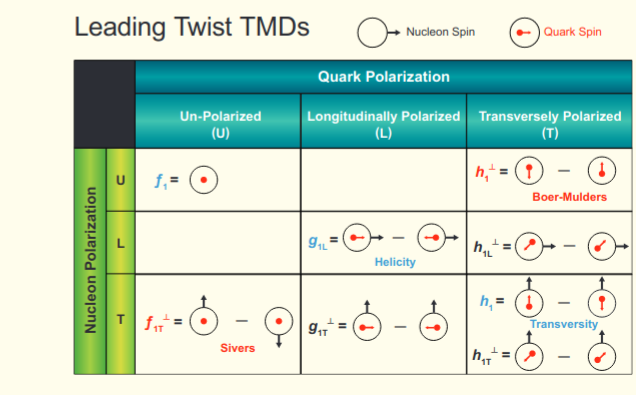
\includegraphics[width=6.cm]{imgs/TMD.png}
\end{Pic}

\begin{List}{9.}{(0.1, 11.)}

  \item  TMDs : distributions of the hadron's quark or gluon momenta that are perpendicular to the momentum transfer between the beam and the hadron.
\end{List}

\end{frame}

\subsection{Boer-Mulders Function \& Drell-Yan Process}

\begin{frame}
\frametitle{Boer-Mulders Function \& Drell-Yan Process}

\begin{Pic}{6.5}{(0.1, 1.)}
  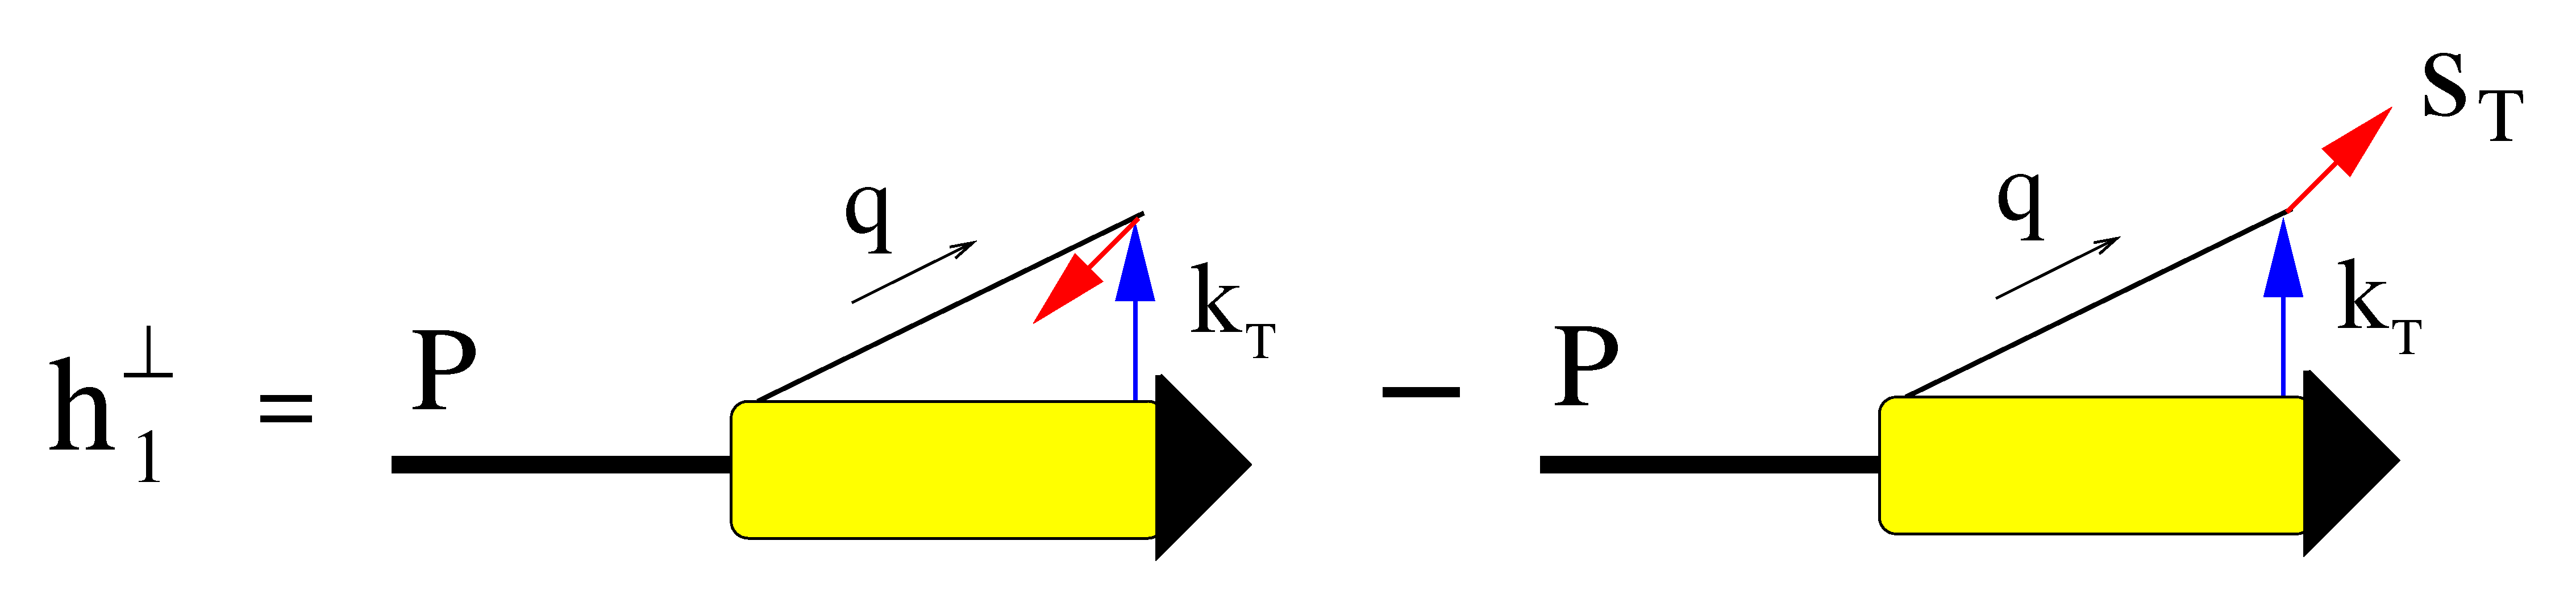
\includegraphics[width=6.5cm]{imgs/BMF.png}
\end{Pic}

\begin{List}{7.}{(0.1, 5.)}

  \item BMF : Describes the net polarization of quarks inside an unpolarized proton.

  \item $h_{1}^{\perp}$ $\rightarrow$ quark distribution that quantifies a particular spin-orbit correlation.

\end{List}

\begin{Pic}{7.0}{(0.1, 10.)}
  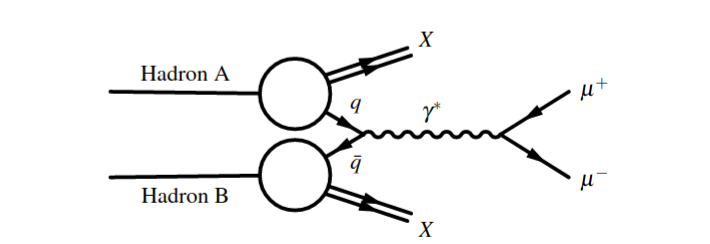
\includegraphics[width=7.cm]{imgs/drell-yan.png}
\end{Pic}

\begin{textblock}{8.}(7., 1.)
\begin{equation*}
\frac{d\sigma}{d\Omega} \propto 1  + \lambda \cos^{2}\theta + \mu \sin 2 \theta \cos \phi + \frac{1}{2}\nu \sin^{2}\theta \cos 2 \phi
\end{equation*}
\end{textblock}

\begin{Pic}{4.7}{(8, 2.5)}
  \NewCaption{J. C. Peng et al.}{https://arxiv.org/abs/1808.04398}{arXiv:1808.04398}
  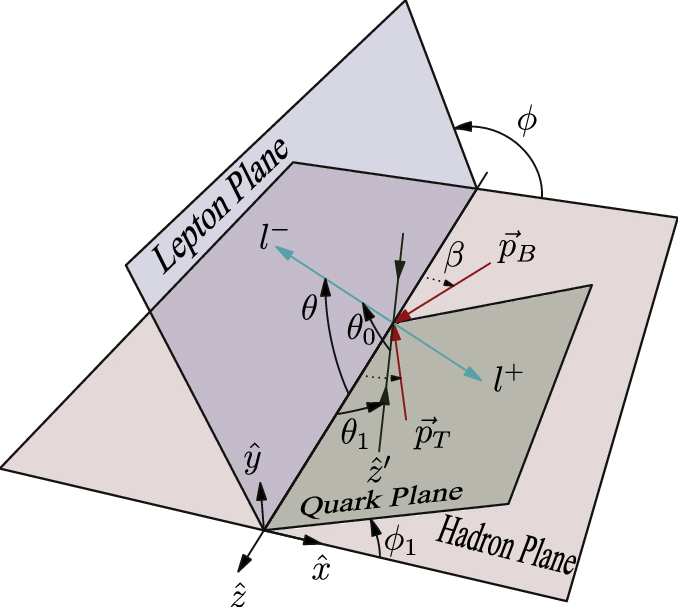
\includegraphics[width=4.7cm]{imgs/three_plane_newest.png}
\end{Pic}

% \begin{scriptsize}
\begin{List}{9.}{(6., 12.)}

  \item Collins-Soper frame: rest frame of di-muons $\rightarrow$ using the beam proton direction to construct the azimuthal and polar angles.

  \item Extraction of the $\nu$ parameter $\rightarrow$ BM function.

\end{List}
% \end{scriptsize}
\end{frame}

\section{FermiLab SeaQuest/E906 Experiment}

\begin{frame}
\frametitle{FermiLab SeaQuest/E906 Experiment}

\begin{Pic}{6.}{(0.5, 1.)}
  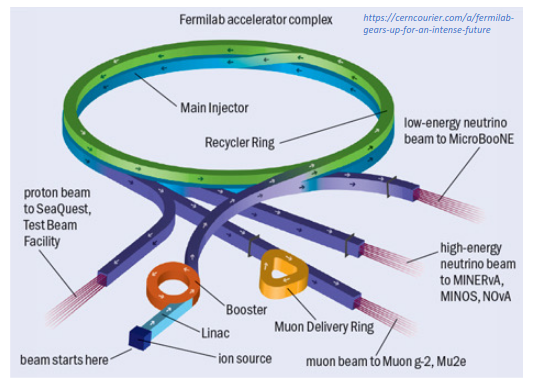
\includegraphics[width=6.cm]{imgs/injector.png}
\end{Pic}

\begin{Pic}{7.5}{(8., 0.01)}
  \NewCaption{C. A. Aidala et al.}{https://arxiv.org/abs/1706.09990}{arXiv:1706.09990}
  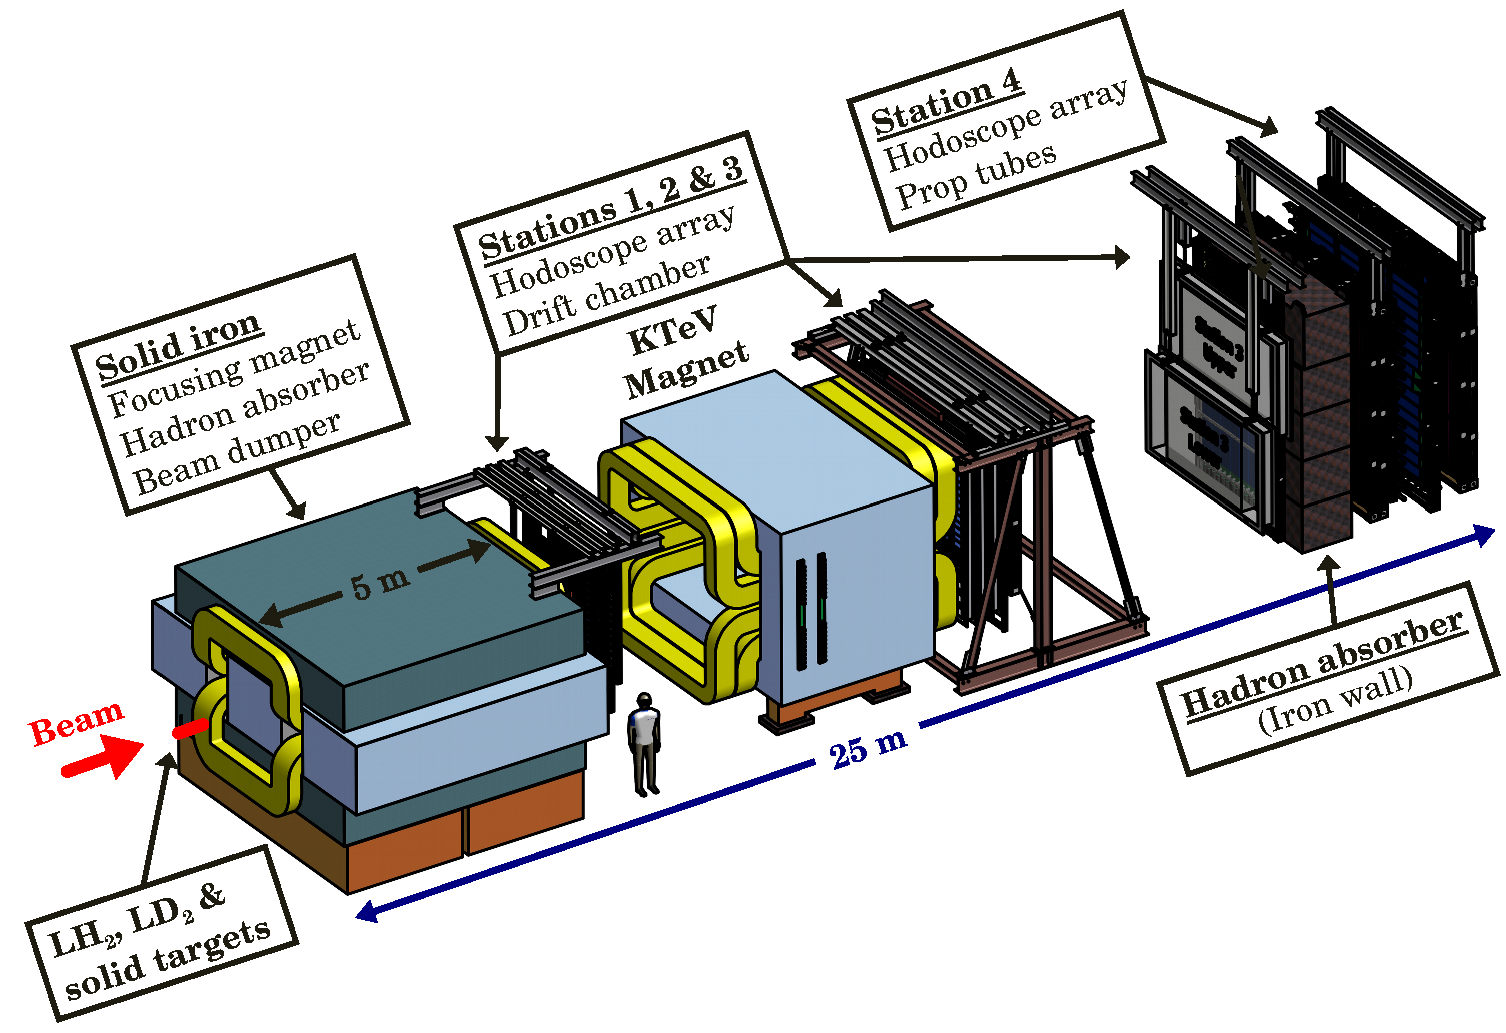
\includegraphics[width=7.5cm]{imgs/spectrometer.pdf}
\end{Pic}

\begin{Pic}{6.5}{(9.5, 8.5)}
  \NewCaption{Nagai, Kei}{https://lss.fnal.gov/archive/thesis/2000/fermilab-thesis-2017-05.pdf}{DOI:10.2172/1346822}
  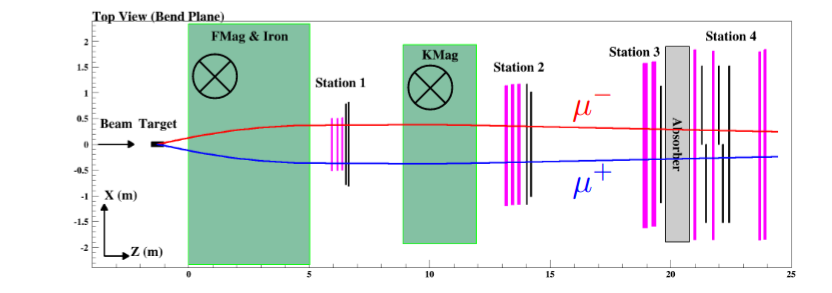
\includegraphics[width=6.5cm]{imgs/mup_mum.png}
\end{Pic}

\begin{Pic}{6.5}{(0.1, 8.5)}
  \NewCaption{J. Dove et al.}{https://arxiv.org/abs/2103.04024}{arXiv:2103.04024}
  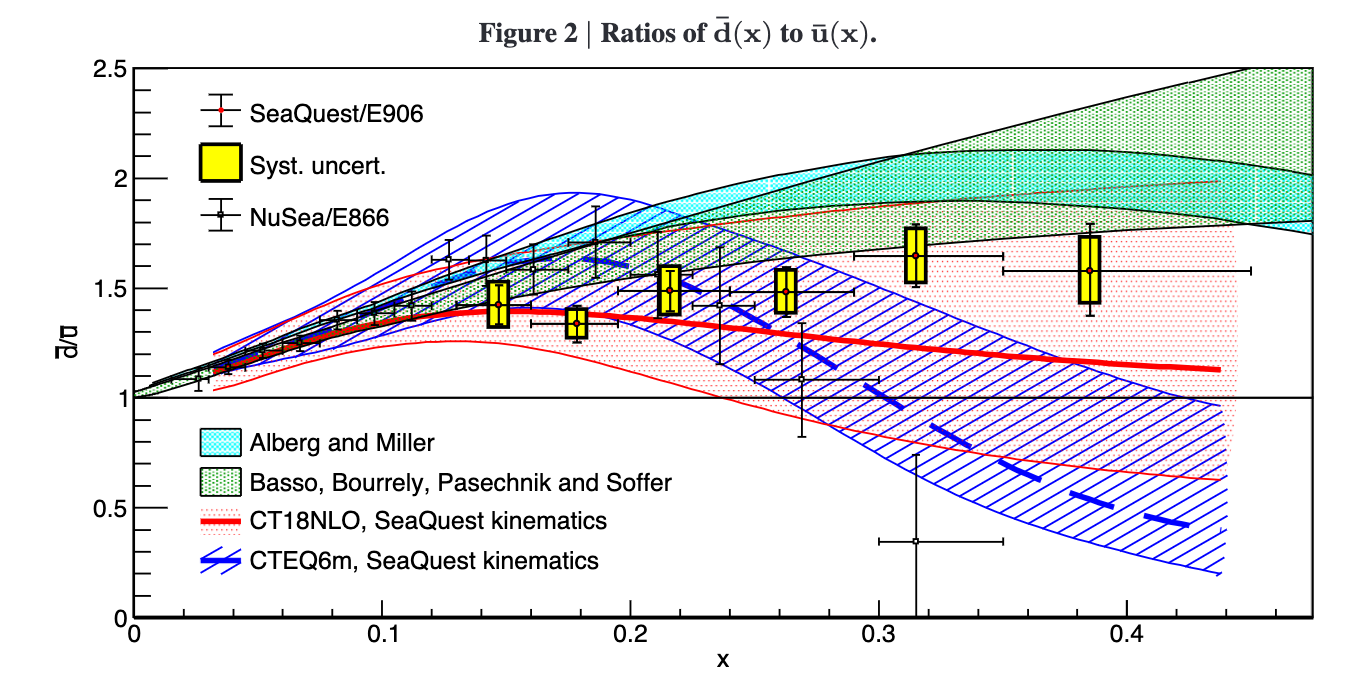
\includegraphics[width=6.5cm]{imgs/ubardbar.png}
\end{Pic}

\begin{scriptsize}
\begin{List}{9.}{(7., 14.)}
  \item Fixed target experiment at FermiLab.

  \item Use 120 GeV beam energy from main injector.
\end{List}
\end{scriptsize}
\end{frame}

\section{Analysis Motivation}
\subsection{Unfolding Detector Level Data}

\begin{frame}
\frametitle{Unfolding Detector Level Data}

\begin{Pic}{7.}{(0.5, 1.)}
  \caption{Particle level data}
  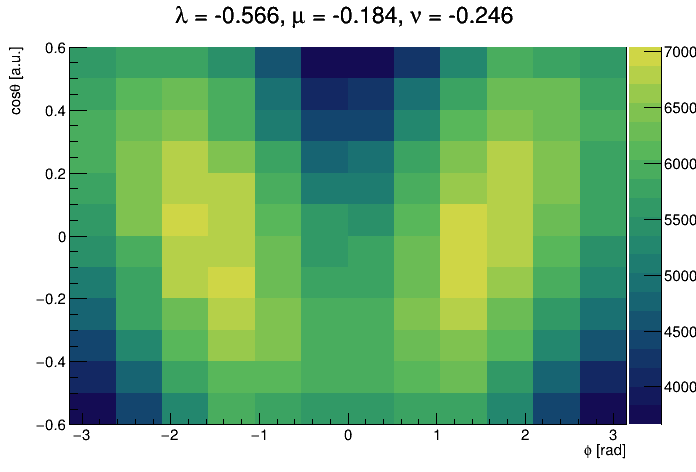
\includegraphics[width=7.cm]{imgs/particle_level.png}
\end{Pic}

\begin{Pic}{7.}{(8., 1.)}
  \caption{Detector level data}
  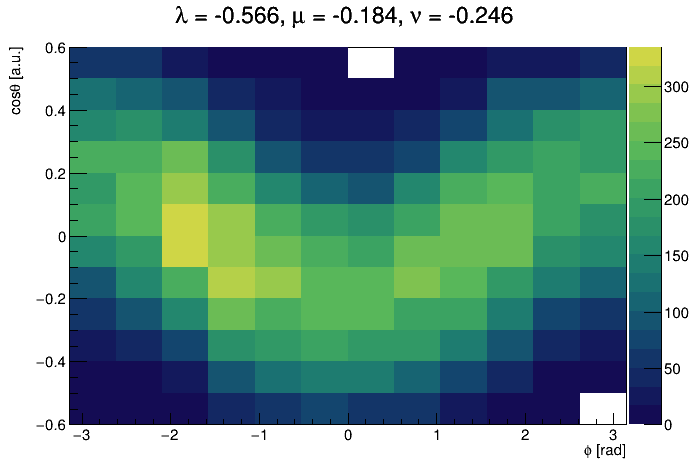
\includegraphics[width=7.cm]{imgs/detector_level.png}
\end{Pic}

\begin{List}{15.}{(0.5, 11.)}

  \item Detector level data need to be corrected for acceptance, reconstruction inefficiencies, detector smearing, etc.

  \item Unfolding $\rightarrow$ $f: X_{\text{detector}} \rightarrow X_{\text{particle}}$

  \item Deep neural networks excel at approximating complex non-linear functions, making them ideal for mapping between detector level and particle level.
\end{List}

\end{frame}

\subsection{Autoencoders and U-Nets}

\begin{frame}
\frametitle{Autoencoders and U-Nets}

\begin{Pic}{7.}{(0.5, 1.)}
  \NewCaption{Taoli Cheng et al.}{https://arxiv.org/abs/2007.01850}{arXiv:2007.01850}
  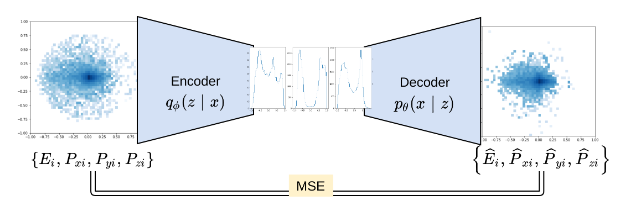
\includegraphics[width=7.cm]{imgs/ae.png}
\end{Pic}

\begin{Pic}{7.}{(8., 1.)}
  \NewCaption{Olaf Ronneberger et al.}{https://arxiv.org/abs/1505.04597}{arXiv:1505.04597}
  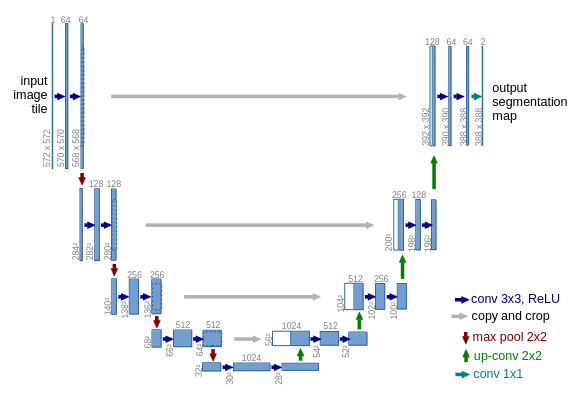
\includegraphics[width=7.cm]{imgs/unet.png}
\end{Pic}

\begin{List}{8.0}{(0.5, 6.5)}

  \item Autoencoders(AE) are generative models, which are also used for image denoising.

  \item AEs encode input data to latent dimension $(z)$ and then decoder try to reconstruct input data.

\end{List}

\begin{List}{15.}{(0.5, 11.2)}

  \item U-Nets are U-shaped AEs that made a major breakthrough in image segmentation.

  \item We use U-Nets to reconstruct particle-level data using detector-level data as inputs.

\end{List}
\end{frame}

\subsection{Data Creation}

\begin{frame}
\frametitle{Data Creation}

\begin{Pic}{5.5}{(9.5, 0.5)}
  \NewCaption{J. Dove et al.}{https://arxiv.org/abs/2103.04024}{arXiv:2103.04024}
  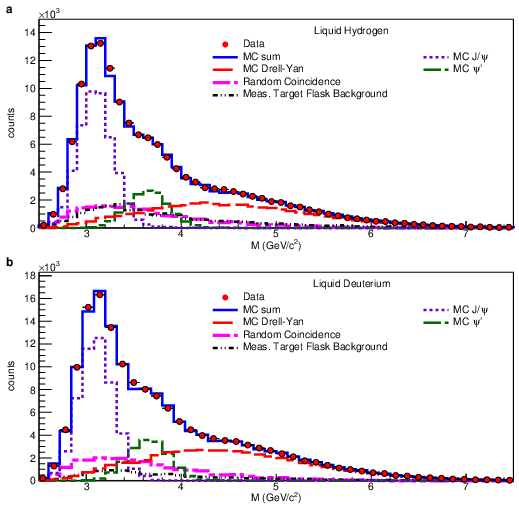
\includegraphics[width=5.5cm]{imgs/mc2real.png}
\end{Pic}

\begin{List}{9.}{(0.1, 2.0)}

  \item Monte-Carlo data was generated using ``PYTHIA" generator and events were passed trough E906 detector simulation using ``GEANT4".

  \item Each histogram has specific $\lambda$, $\mu$, and $\nu$ values, which were sampled uniformly from the ranges [-1, 1], [-0.5, 0.5], and [-0.5, 0.5] respectively.

  \item DY angular coefficients were injected to a histograms by weighting the events using;

  \begin{equation*}
w = \frac{1  + \lambda \cos^{2}\theta + \mu \sin 2 \theta \cos \phi + \dfrac{1}{2}\nu \sin^{2}\theta \cos 2 \phi}{1 + \cos^{2}\theta}
  \end{equation*}

\end{List}
\end{frame}

\subsection{U-Net Architecture}

\begin{frame}
\frametitle{U-Net Architecture}

\begin{Pic}{12.}{(0.1, -1.)}
  \includegraphics[width=12.cm]{imgs/U_net_arch.png}
\end{Pic}

\begin{textblock}{11.}(4., 15.)
\begin{scriptsize}
Model was trained in  Fermilab Elastic Analysis Facility (\textcolor{blue}{\href{https://eafjupyter.readthedocs.io/en/latest/index.html}{EAF}}) using Nvidia A100 GPU.
\end{scriptsize}
\end{textblock}

\end{frame}

\subsection{Unfolded Results}

\begin{frame}
\frametitle{Few Unfolded Histograms}

\begin{Pic}{6.}{(0.5, 1.)}
  \caption{Particle level}
  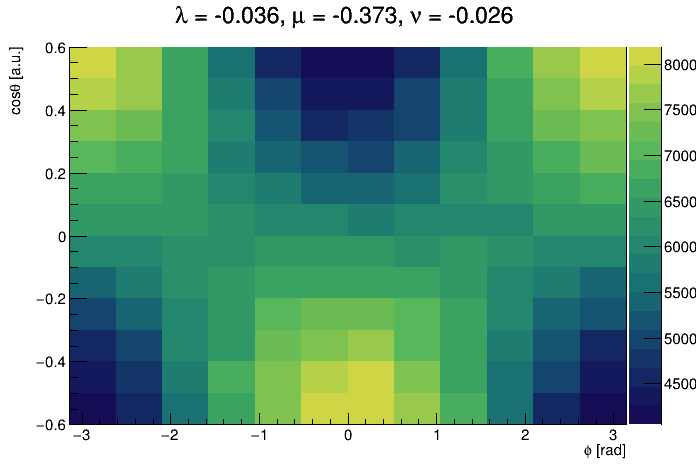
\includegraphics[width=6.cm]{imgs/true_fit_1.png}
\end{Pic}

\begin{Pic}{5.}{(0.5, 8.5)}
  \caption{Detector level}
  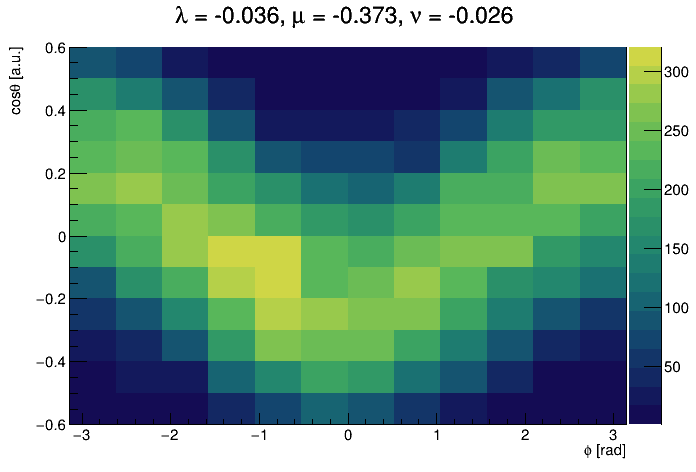
\includegraphics[width=5.cm]{imgs/reco_fit_1.png}
\end{Pic}

\begin{Pic}{8.}{(7., 2.)}
  \caption{Unfolded}
  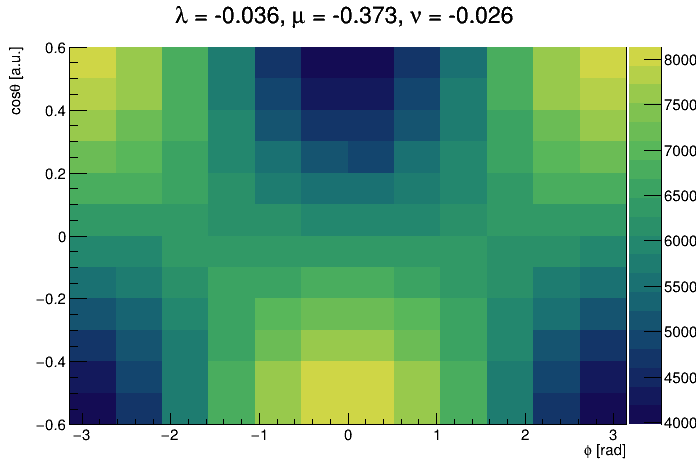
\includegraphics[width=8.cm]{imgs/pred_fit_1.png}
\end{Pic}

\begin{textblock}{8.}(7., 14.)
\begin{scriptsize}
Note that particle level - generated truth info., detector level - reconstruct info., unfolded - U-Net output
\end{scriptsize}
\end{textblock}

\end{frame}


\begin{frame}
\frametitle{Few Unfolded Histograms}

\begin{Pic}{6.}{(0.5, 1.)}
  \caption{Particle level}
  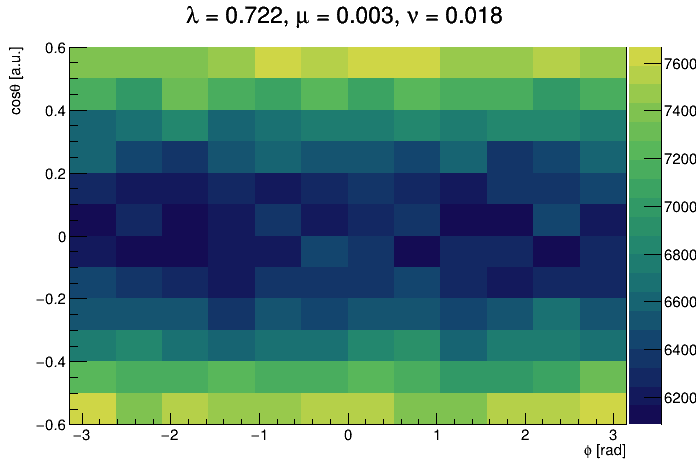
\includegraphics[width=6.cm]{imgs/true_fit_2.png}
\end{Pic}

\begin{Pic}{5.}{(0.5, 8.5)}
  \caption{Detector level}
  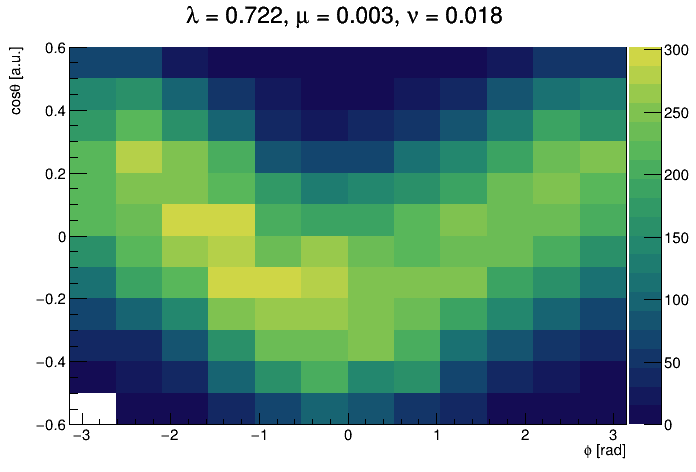
\includegraphics[width=5.cm]{imgs/reco_fit_2.png}
\end{Pic}

\begin{Pic}{8.}{(7., 2.)}
  \caption{Unfolded}
  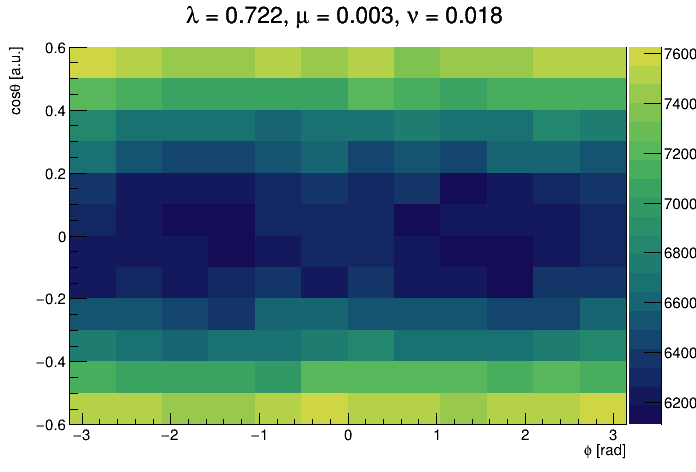
\includegraphics[width=8.cm]{imgs/pred_fit_2.png}
\end{Pic}
\end{frame}

\begin{frame}
\frametitle{Few Unfolded Histograms}

\begin{Pic}{6.}{(0.5, 1.)}
  \caption{Particle level}
  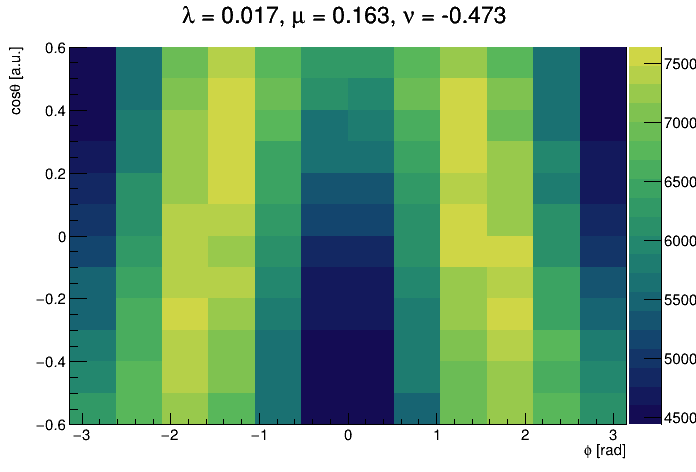
\includegraphics[width=6.cm]{imgs/true_fit_3.png}
\end{Pic}

\begin{Pic}{5.}{(0.5, 8.5)}
  \caption{Detector level}
  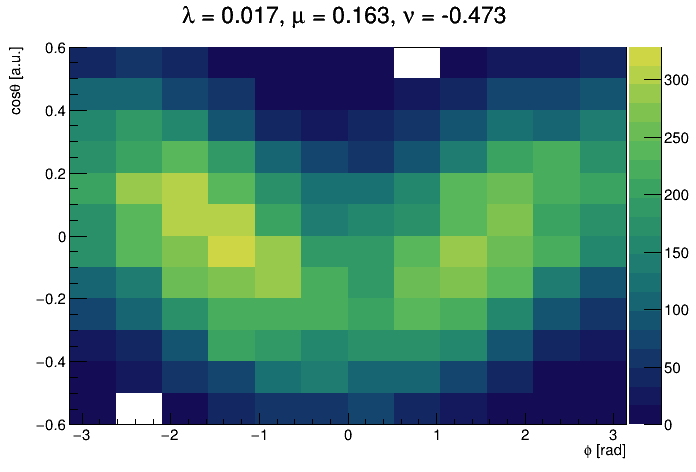
\includegraphics[width=5.cm]{imgs/reco_fit_3.png}
\end{Pic}

\begin{Pic}{8.}{(7., 2.)}
  \caption{Unfolded}
  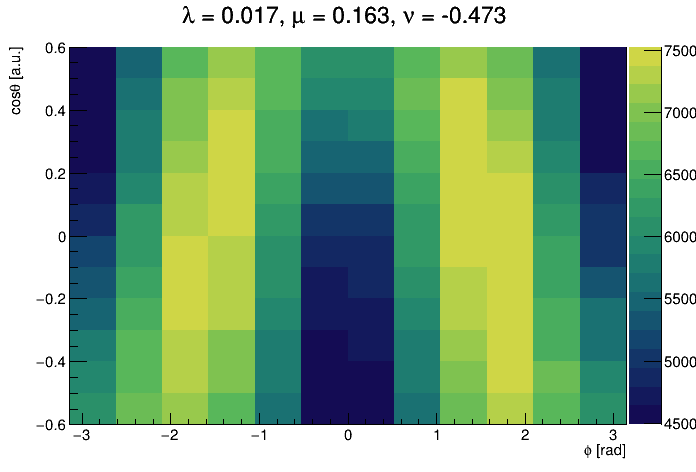
\includegraphics[width=8.cm]{imgs/pred_fit_3.png}
\end{Pic}
\end{frame}

\begin{frame}
\frametitle{Resolution of the Unfolded Fit Results}

\begin{Pic}{5.5}{(0.5, 1.)}
  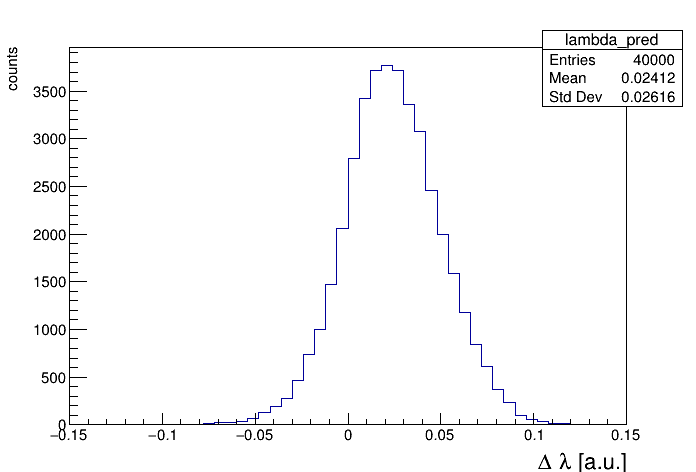
\includegraphics[width=5.5cm]{imgs/lambda_pred.png}
\end{Pic}

\begin{Pic}{5.5}{(7.0, 1.)}
  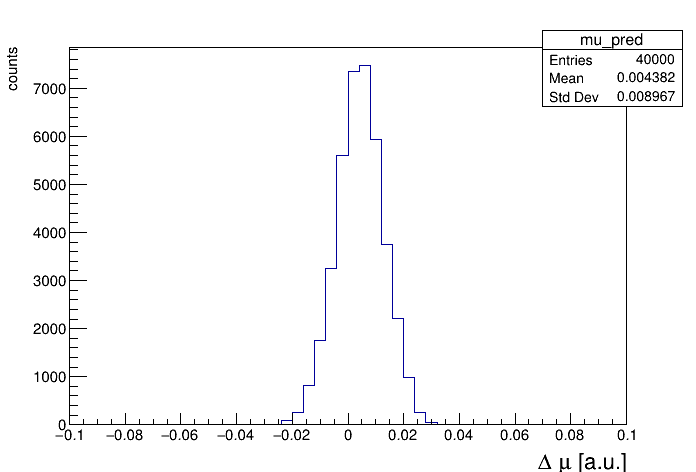
\includegraphics[width=5.5cm]{imgs/mu_pred.png}
\end{Pic}

\begin{Pic}{5.5}{(0.5, 8.)}
  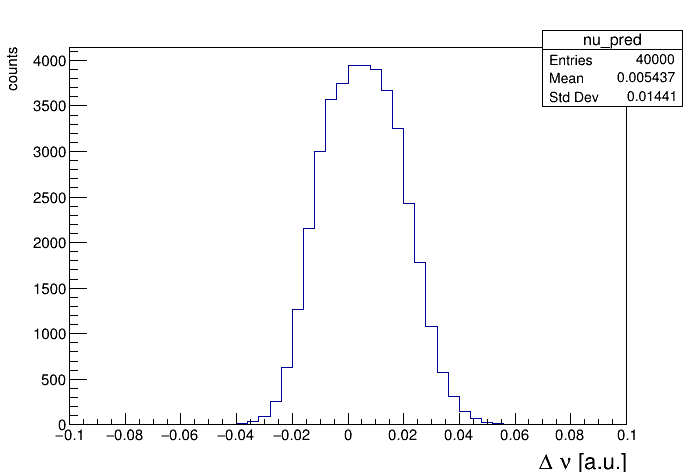
\includegraphics[width=5.5cm]{imgs/nu_pred.png}
\end{Pic}

\begin{List}{9.0}{(6.5, 9.)}

  \item Unfolded $\phi$-$\cos\theta$ histograms are fitted using;

\begin{scriptsize}
\begin{equation}
\label{eq:1}
f(\phi, \cos\theta) = A(1  + \lambda \cos^{2}\theta + \mu \sin 2 \theta \cos \phi + \dfrac{1}{2}\nu \sin^{2}\theta \cos 2 \phi)
\end{equation}
\end{scriptsize}

  \item X axis;  $\Delta = \text{Injected} - \text{Unfolded}$

\end{List}
\end{frame}

\begin{frame}
\frametitle{Comparison of Few Unfolded Fit Results}

\begin{textblock}{15.}(0.5, 2.)
\begin{center}
% \begin{tabular}{|c c c c|}
% \hline
%  & Injected & Particle level & Unfolded \\
% \hline
% $\lambda$ & -0.566 & -0.584 $\pm$ 0.008 & -0.579 $\pm$ 0.007 \\
% $\mu$ & -0.184 & -0.178 $\pm$ 0.002 & -0.177 $\pm$ 0.002 \\
% $\nu$ & -0.246 & -0.238 $\pm$ 0.003 & -0.241 $\pm$ 0.003 \\
% \hline
% $\lambda$ & -0.036 & -0.037 $\pm$ 0.009 & -0.035 $\pm$ 0.009 \\
% $\mu$ & -0.373 & -0.367 $\pm$ 0.002 & -0.370 $\pm$ 0.002 \\
% $\nu$ & -0.026 & -0.021 $\pm$ 0.003 & -0.033 $\pm$ 0.003 \\
% \hline
% $\lambda$ & 0.722 & 0.701 $\pm$ 0.011 & 0.689 $\pm$ 0.011 \\
% $\mu$ & 0.003 & 0.006 $\pm$ 0.002 & -0.004 $\pm$ 0.002 \\
% $\nu$ & 0.018 & 0.016 $\pm$ 0.003 & 0.019 $\pm$ 0.003 \\
% \hline
% \end{tabular}

\begin{tabular}{|c c c|}
\hline
 & Particle level & Unfolded \\
\hline
$\lambda$ & -0.584 $\pm$ 0.008 & -0.579 $\pm$ 0.007 \\
$\mu$ & -0.178 $\pm$ 0.002 & -0.177 $\pm$ 0.002 \\
$\nu$ & -0.238 $\pm$ 0.003 & -0.241 $\pm$ 0.003 \\
\hline
$\lambda$ & -0.037 $\pm$ 0.009 & -0.035 $\pm$ 0.009 \\
$\mu$ & -0.367 $\pm$ 0.002 & -0.370 $\pm$ 0.002 \\
$\nu$ & -0.021 $\pm$ 0.003 & -0.033 $\pm$ 0.003 \\
\hline
$\lambda$ & 0.701 $\pm$ 0.011 & 0.689 $\pm$ 0.011 \\
$\mu$ & 0.006 $\pm$ 0.002 & -0.004 $\pm$ 0.002 \\
$\nu$ & 0.016 $\pm$ 0.003 & 0.019 $\pm$ 0.003 \\
\hline
\end{tabular}
\end{center}
\end{textblock}

\begin{scriptsize}
\begin{List}{15.}{(0.5, 13.)}
  \item Note that these $\lambda$, $\mu$, and $\nu$ values does not represent any physics information.

  \item To extract the $\lambda$, $\mu$, and $\nu$ values, a fit was performed using equation \ref{eq:1} for both particle and detector levels.
\end{List}
\end{scriptsize}

\end{frame}

\section{Summary}

\begin{frame}
\frametitle{Summary}

\begin{List}{15.}{(0.5, 2.)}

  \item The spin of the proton is an intrinsic property that can be used to understand the internal structure of the proton.

  \item A non-zero $\cos2\phi$ asymmetry in the Drell-Yan process will provide information about the transverse motion of the quarks inside the proton.

  \item U-Nets can be utilized as a method to unfold detector-level data to particle-level data. This approach is applicable in high-dimensional feature spaces.

  \item We plan to use this method to extract the Drell-Yan angular coefficients from the FermiLab E906/SeaQuest data with higher  precision.

  \item We plan to correct any discrepancies between experimental data and Monte Carlo (MC) simulations by reweighting.

  \item We plan to use the ``Bootstrapping" method to enhance the precision of the prediction.

  \item Acknowledgment: This work was funded by the DOE Office of Science, Medium-Energy Nuclear Physics Program.

\end{List}

\end{frame}

\end{document}
